\chapter{Constraints \& Justification \\
  \small{\textit{-- Evan Ciok, Sophia DiCuffa, Carson McManus}}
  \index{Chapter!constraints}
  \index{Chapter!justification}
  \label{Chapter::ConstraintsJustification}}


TODO: describe any system constraints

TODO: describe justification for why leader election will be too complex

\section{Browser Websocket API Contraints}

The Websocket API allows for one to open a bidirectional communication session between a browser and a server. The connection session stays open until the browser or server terminates it. 
This allows for the client and server to send information to the other simultaneously. The browser's API does not allow custom HTTP headers, which means that authorization has to be done after the connection request has been made \cite{MDNWebSocket} \cite{HerokuWebSocket}.

\subsection{Issues with Stateless Balancer}

The load balancer must be able to maintain the list of which rooms each monolith node has loaded. If this does not happen, clients who join the same room will load different instances of the room across different nodes, resulting in state fragmentation. The sequence diagram for multiple clients joining the same room through a normal, stateless load balancer is shown below in figure \ref{Figure::join-room-stateless} to illustrate this issue.

\begin{figure}[!htb]
  \centering
  \scalebox{0.57}{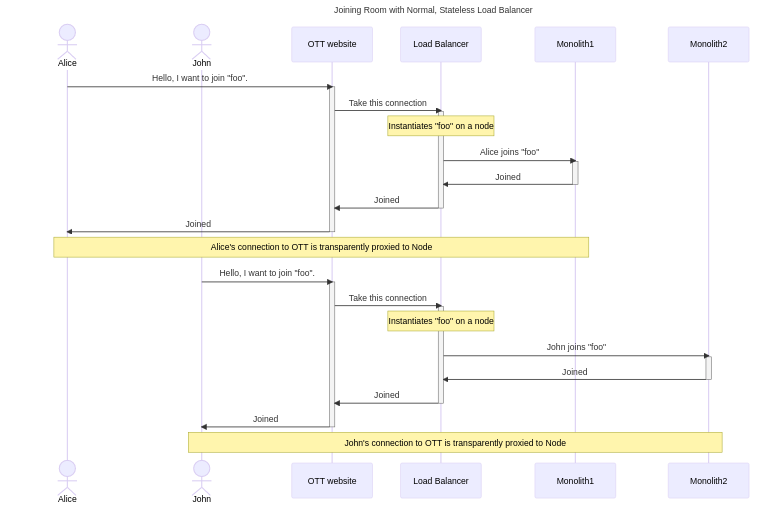
\includegraphics{Figures/join-room-stateless.png}}
  \caption{\label{Figure::join-room-stateless} Sequence Diagram for Room Loading on Stateless Balancer.}
\end{figure}


\section{Balancer Must Use Asynchronous I/O \index{async} \index{asynchronous I/O} \index{io}}

The Balancer's workload is I/O bound, and it must be able to handle many concurrent network connections. For I/O bound workloads, it's more performant to use asynchronous I/O\cite{async-vs-threads}.

\section{Current Deployments Must Continue to Work}

Once the load balancer is implemented, the current deployments of OTT must continue to function as intended. Likewise, any updates to the Monolith should not affect the functionality of current deployments.

\section{Deployment Must Work Without Load Balancer}

Not all self-hosters of OTT might want the added complexity of the load balancer, so it must remain possible to deploy OTT without it. It would also be beneficial to be able to quickly reroute traffic between the balancer and the monolith during the initial deployment stage.